\documentclass[../../main.tex]{subfiles}

\graphicspath{{\subfix{../../immagini/}}}

\begin{document}

I metodi introdotti nei precedenti paragrafi, come già accennato, risultano in molti contesti fortemente limitati nel tipo di pattern che possono descrivere, per questo motivo si rendono necessari modelli più espressivi per poter approssimare funzioni più complesse.

Introduciamo quindi il concetto di \textit{rete neurale artificiale}, concentrandoci poi su due specifiche architetture di reti: \textit{percettroni multistrato} e \textit{reti ricorrenti}, che saranno quelle utilizzate negli esperimenti descritti nel Capitolo \ref{chap:Esperimenti}.  

Formalmente, una rete neurale è una tripla $(N, V, w)$, dove $N$ rappresenta l'insieme di neuroni, o unità, della rete, $V \subset N \times N$ è un insieme della forma $\{(i, j) | i,j \in N\}$ e rappresenta le connessioni tra le unità della rete $i$ e $j$ e $w$ è una funzione definita come:
\[w : V \rightarrow \mathbb{R},\]
che rappresenta il peso di una connessione $(i, j)$ \cite{kriesel2007bin}.

\begin{figure}[H]
    \centering
    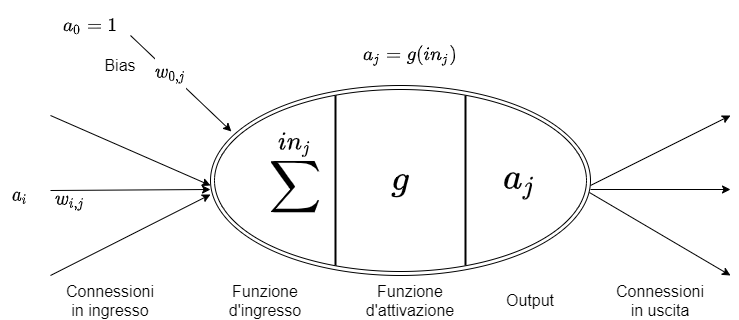
\includegraphics[width=\textwidth]{immagini/4_2/neuron.png}
    \caption{Struttura di un neurone}
    \label{fig:neuron}
\end{figure}

Ogni neurone risulta collegato con una serie di altre unità ricevendo in ingresso i rispettivi output che trasforma in base al valore dei relativi pesi $w((i,j))$, una volta prodotto l'output questo viene a sua volta propagato ad una serie di altri neuroni.

Formalmente, posso suddividere la struttura di un neurone $j$ in diverse parti (Figura \ref{fig:neuron}): ogni valore ricevuto in ingresso prende il nome di attivazione $a_i$, questi vengono prima passati attraverso una funzione d'ingresso, che spesso viene definita come somma pesata dei valori d'ingresso:
\[in_j = \sum_{i=0}^n {w_{i,j} a_i},\]
la notazione $w_{i,j}$ indica il valore del peso $w((i,j))$ tra due neuroni $i$ e $j$. Il risultato della funzione d'ingresso viene poi fornito in input alla funzione d'attivazione $g$:
\[a_j = g(in_j),\]
infine, il valore d'attivazione viene passato attraverso una funzione di output che in molti casi semplicemente corrisponde ad una funzione identità:
\[f_{out}(a_j) = a_j,\]
il valore $a_j$ prodotto viene poi propagato ai neuroni dei livelli successivi.

In generale la funzione d'attivazione può avere diverse forme, la Figura \ref{fig:activations} mostra alcune delle più comuni.

\begin{figure}[H]
    \centering
    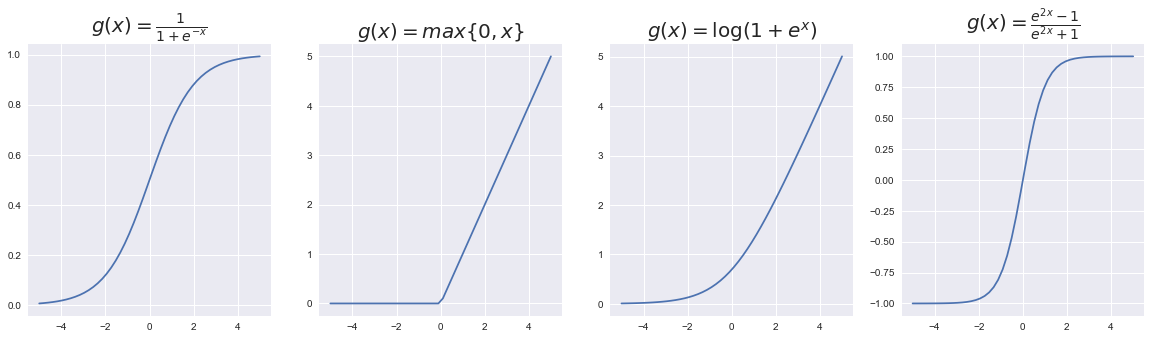
\includegraphics[width=\textwidth]{immagini/4_2/activation_func.png}
    \caption{Esempi di tipiche funzioni d'attivazione}
    \label{fig:activations}
\end{figure}

L'aspetto che rende le reti neurali modelli in genere più espressivi rispetto ad approcci come regressione lineare o logistica, definiti nei paragrafi precedenti, è il fatto di poter connettere più unità funzionali tra di loro, questa caratteristica permette di creare funzioni d'ipotesi $h$ esprimibili come risultato della composizione di molteplici funzioni $f$:
\[h(\boldsymbol{x}) = f_k\left(f_2\left(f_1(\boldsymbol{x})\right)\right).\]

Per  `sfruttare' a pieno questa caratteristica è però importante che le funzioni d'attivazione $g$ siano:
\begin{itemize}
    \item \textit{non lineari}: altrimenti l’uscita della rete sarebbe sempre lineare e il modello sarebbe troppo semplice,
    \item \textit{differenziabili}: per facilitare l'applicazione di algoritmi basati sulla discesa del gradiente.
\end{itemize}

Una volta definita la struttura di un neurone è utile analizzare come più neuroni possono connettersi per andare a formare la rete: le due tipologie di architettura utilizzate negli esperimenti del Capitolo \ref{chap:Esperimenti} sono la rete feed forward (Figura \ref{fig:feedforward}) e la rete ricorrente (Figura \ref{fig:RNN}). Indipendentemente dal tipo di architettura, considereremo qui solamente reti organizzate a strati. Ogni rete di questo tipo è composta da due o più livelli, o strati: ogni livello conterrà uno o più neuroni connessi con uno o più neuroni dello stesso o di altri strati; le connessioni possibili di un neurone appartenente ad uno specifico strato sono dettate dalla tipologia di architettura considerata. Il primo e l'ultimo strato di una rete prendono rispettivamente il nome di strato d'ingresso e strato d'uscita, tutti gli strati compresi tra questi due prendono il nome di strati nascosti.

Intuitivamente, tramite la composizione di molteplici $f$ è possibile creare funzioni d'ipotesi $h$ in grado di approssimare funzioni complesse; questa intuizione, oltre ad essere corretta, viene formalizzata nel \textit{teorema di approssimazione universale} \cite{journals/mcss/Cybenko89}, che dimostra un risultato ancora più forte: una rete feedforward composta da un singolo strato nascosto con un numero arbitrario e finito di neuroni e con una funzione logistica (Figura \ref{fig:activations}) come funzione d'attivazione è in grado di approssimare con precisione arbitraria una qualsiasi funzione continua.

\begin{figure}[H]
    \begin{subfigure}[]{0.48\textwidth}
        \centering
        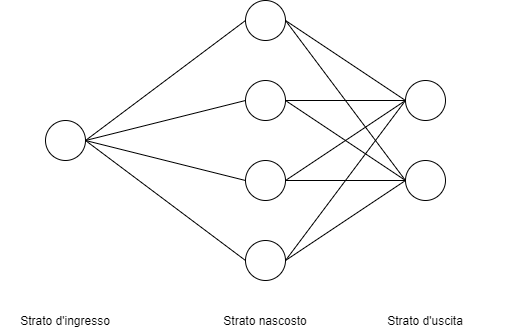
\includegraphics[width = \textwidth]{immagini/4_2/feed_forward.png}
        \caption{Esempio di rete neurale con architettura feed forward}
        \label{fig:feedforward}        
    \end{subfigure}
    \begin{subfigure}[]{0.48\textwidth}
        \centering
        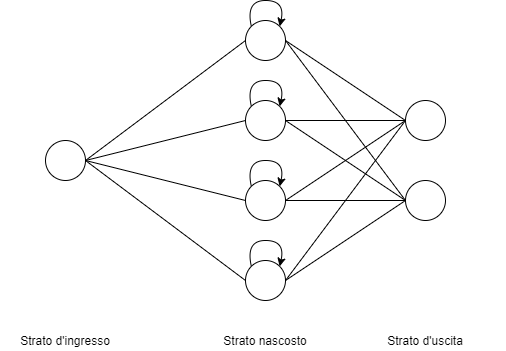
\includegraphics[width = \textwidth]{immagini/4_2/RNN.png}
        \caption{Esempio di rete neurale ricorrente, in questo caso la ricorrenza è solamente diretta}
        \label{fig:RNN}
    \end{subfigure}
    \caption{}
\end{figure}

Una \textit{rete feedforward} è composta da un livello d'ingresso, uno d'uscita e da uno o più livelli nascosti. Le connessioni in questa topologia sono permesse solo tra neuroni di livelli consecutivi. Dato un elemento del dataset $\boldsymbol{x}$ la relativa predizione viene generata passando al livello d'ingresso il vettore $\boldsymbol{x}$, il livello d'uscita conterrà quindi la predizione $h(\boldsymbol{x})$, risultato della composizione delle funzioni di ognuno degli strati. Se il numero di livelli nascosti è superiore a 3 si parla di reti profonde.

Una \textit{rete ricorrente} è una tipologia in cui sono permesse connessioni tra neuroni che generano cicli: parlo nello specifico di ricorrenza diretta nel caso in cui un neurone sia connesso con se stesso, di ricorrenza indiretta quando sono ammesse connessioni verso livelli precedenti e di ricorrenza laterale quando sono ammessi connessioni tra neuroni dello stesso strato. A differenza quindi di ciò che accade con una topologia feedforward, nel caso di una rete ricorrente il risultato di un determinato input può essere funzione degli input precedenti. Reti che sfruttano questa architettura quindi supportano possono avere una sorta di `memoria a breve termine', ciò li rende modelli più interessanti per alcuni problemi, ma ovviamente anche più complessi.

\end{document} 